159. \begin{figure}[ht!]
\center{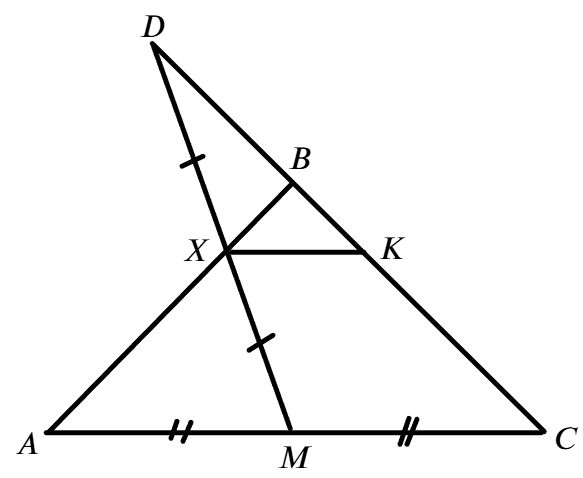
\includegraphics[scale=0.35]{g7-156.png}}
\end{figure}\\
Пусть точка $K$ --- середина $DC.$ Тогда отрезок $XK$ является средней линий треугольника $DMC,$ поэтому $XK\parallel MC.$ Тогда из равенства соответственных углов при секущей $XK$ получим соотношение $\angle BXK=\angle A=\angle C=\angle BKX,$ а значит треугольник $XBK$ является равнобедренным. Тогда $KC=BC-BK=AB-BX=AX,$ поэтому $2AX=2KC=CD,$ ч.т.д.
\end{document}
